\documentclass[conference]{IEEEtran}
%\IEEEoverridecommandlockouts
% The preceding line is only needed to identify funding in the first footnote. If that is unneeded, please comment it out.

%JAMES - BEGIN
\usepackage{glossaries}
% Não é necessário ordenar as siglas
% Example of use: 
% \acrfull{SOA} 
%	Display: Software-Oriented Architecture (SOA)
% \acrshort{SOA}
%	Display: SOA
% \acrlong{SOA}
%	Display: Software-Oriented Architecture

\newcommand{\sigla}[2]{\newacronym{#1}{#1}{#2}}%

\sigla{SLR}{Systematic Literature Review}
\sigla{SOA}{Service-Oriented Architecture}
\sigla{SBA}{Service-Based Architecture}
\sigla{SOC}{Service-Oriented Computing}
\sigla{REST}{Representational State Transfer}
\sigla{SOAP}{Simple Object Access Protocol}
\sigla{XP}{Extreme Programming}
\sigla{FDD}{Feature-Driven Development}
\sigla{DSDM}{Dynamic Systems Development Method}
\sigla{RUP}{Rational Unified Process}
\sigla{ASD}{Adaptive Software Development}
\sigla{ISD}{Internet Speed Development}
\sigla{PP}{Pragmatic Programming}
\sigla{IT}{Information Technology}


\newcommand{\citet}[1]{\cite{#1}}%
\usepackage[colorinlistoftodos]{todonotes}
%JAMES - END

\usepackage{cite}
\usepackage{amsmath,amssymb,amsfonts}
\usepackage{algorithmic}
\usepackage{graphicx}
\usepackage{textcomp}
\usepackage{xcolor}
\def\BibTeX{{\rm B\kern-.05em{\sc i\kern-.025em b}\kern-.08em
    T\kern-.1667em\lower.7ex\hbox{E}\kern-.125emX}}
\begin{document}


\title{A systematic literature review for agile development processes in a service-oriented architecture environment
\thanks{Identify applicable funding agency here. If none, delete this.}
}

\author{\IEEEauthorblockN{1\textsuperscript{st} James Taylor Faria Chaves}
\IEEEauthorblockA{\textit{Postgraduate Program in Applied Computing (PPCA)} \\
\textit{University of Brasilia (UNB)}\\
Brasilia, Brazil \\
jameschaves@gmail.com}
\and
\IEEEauthorblockN{2\textsuperscript{nd} Sergio Antônio Andrade de Freitas}
\IEEEauthorblockA{\textit{Postgraduate Program in Applied Computing (PPCA)} \\
\textit{University of Brasilia (UNB)}\\
Brasilia, Brazil \\
sergio.freitas@unb.br}
}

\maketitle

\begin{abstract}
This document is a model and instructions for \LaTeX.
This and the IEEEtran.cls file define the components of your paper [title, text, heads, etc.]. *CRITICAL: Do Not Use Symbols, Special Characters, Footnotes, 
or Math in Paper Title or Abstract.
\end{abstract}

\begin{IEEEkeywords}
component, formatting, style, styling, insert
\end{IEEEkeywords}

\section{Introduction}
\label{sec:Introduction}
Introduction xx xx  

xx
x

x

x

x

x

x

x

x

x



\section{Background}
\label{sec:Background}
\subsection{Systematic Literature Review}
\label{subsec:SLR}
One instrument used to synthesizing evidence in some research area is the \acrfull{SLR} \cite{Petersen2015}. \acrshort{SLR} is a methodologically rigorous review of research results and its main aim is aggregate all existing evidence on a research question and it is initially used in medicine researchers \cite{Kitchenham2009}. \citet{Kitchenham2004} presented the guideline for performing \acrshort{SLR} in Software Engineering that was derived from existing guidelines used by medical researches. According to \citet{Kitchenham2004}:

\textit{``A systematic literature review is a means of identifying, evaluating and interpreting all available research relevant to a particular research question, or topic area, or phenomenon of interest. Individual studies contributing to a systematic review are called primary studies; a systematic review is a form a secondary study.''}

According to \citet{Kitchenham2004}, the \acrshort{SLR} has more scientific value than a simple literature review due to the methodological rigor of \acrshort{SLR}. The reasons to performing a \acrshort{SLR} are to summarize the existing evidence concerning a treatment or technology, to identify any gaps in current research in order to suggest areas for further investigation and to provide a framework/background in order to appropriately position new research activities. 

\subsection{Agile Development}
\label{subsec:AgileDevelopment}
A light method for software development can be understood as a method that the needs and goals of the stakeholders drive the development and enable the rapid and flexible development of software. The processes and tools itself are less important than deliverables, people, developers and stakeholders, communication, and the ability to adapt to change. This type of method has to be iterative, incremental, cooperative and adaptable to changes in environments and requirements \cite{Abdelouhab2014,Chehili2013,Farroha2011}. The search for this type of software development method led to the “agile methods” that were stated in the Agile Manifesto, published in 2001 \cite{alliance2001agile} where seventeen developers and consultants representatives of light methods for software development met to discuss better ways of developing software.

There are many methods of software development that claim to be agile development methods such as SCRUM, \acrfull{RUP}, \acrfull{DSDM}, \acrfull{ASD}, \acrfull{ISD}, Lean, Crystal Clear, \acrfull{XP}, \acrfull{FDD}, \acrfull{PP}, and so on \cite{Carvalho2013,INAYAT2015915,Highsmith2001Agile,DYBA2008833,VallonSLRAgile2018,Timperi2004}. Each of them has its own phases and a life cycle, and some methods do not even define well the stages of development. The following are some characteristics of each of the main of these agile methodologies, according to \citet{Timperi2004}:
\begin{itemize}
\item \acrfull{FDD} is based on several best practices and it emphasizes design and building activities. The requirements are captured first by constructing a domain object model and using it as a basis for requirements elicitation and inspections are the main quality assurance practice but testing is also mandatory.
\item \acrfull{XP} is based on short iterations and incremental development with constant feedback from both the customer and other developers and most of the practices of XP are aimed at quality assurance and in particular getting timely feedback.
\item \acrfull{DSDM} relies heavily on prototyping in most development activities and proposes a pragmatic view to quality; the emphasis is on early validation while technical quality can be sacrificed.
\item SCRUM is based on empirical management and it does not state engineering practices and consists of development in iterations called sprints. The requirements are captured in prioritized order in a product backlog and in a sprint backlog for the current sprint. Daily management is handled by scrum meetings in which participants answer three questions regarding what they have done since the last scrum meeting, what they will do between now and the next scrum meeting, and what problems they have.
\end{itemize}





\subsection{Service-Oriented Architecture}
\label{subsec:SOA}
Organizations have their own business goals and they need software systems to satisfy those goals, sometimes with crosscutting stakeholders concerns. One of the key challenges to building systems that meet the goals of large numbers of stakeholders is integrating and reusing existing systems, while adding new functionality to support the business processes and to respond to changes in the business. Software Architecture is a bridge between those goals and the final resulting system. Software Architecture comprehends the set of structures needed to reason about the system, which comprise software elements, relations among them, and properties of both. In the ending of the 20th century, new approaches to system architecture have emerged which aim to structure a complex system around units of capability, called services \cite{bass2007software,Demchak2007,krogdahl2005service}.

This is the context in which \acrfull{SOA} is placed, that has emerged as a widely accepted solution to this challenge allowing a homogeneous enterprise-wide solution satisfying objectives that include an easy and flexible integration with legacy systems and simplifying business processes. Software architecture can be composed by several design patterns simultaneously to obtain its aim and \acrshort{SOA} is a paradigm, a design pattern, not a complete architecture. This design pattern was already used since the beginning of 1990s, mainly in \acrfull{SOAP} \cite{erl2008soa,ZurMuehlen2005} form. In the middle of 2000 years, the \acrfull{REST} \cite{Severance2015,ZurMuehlen2005} form began to spread and today its hardy do say witch proportion news applications are made in one or other form, existing intermediary forms, between both \cite{ZurMuehlen2005}. \acrshort{SOA} is a sort of architecture that use standards-based infrastructure to forge large-scale systems out of loosely coupled, inter-operable services, distributed, invocable, publishable and business oriented that can act like providers, consumers or \acrfull{IT} elements that join providers and consumers. \acrshort{SOA} can create systems-of-systems by mapping existing systems into services, then orchestrating communication between the services. New functionality can be created by either adding new services or modifying communication among existing services with low costs, innovators services to clients, agile adaption, and reaction to opportunity and weakness competitiveness \cite{bass2007software,Demchak2007,Shi2000,idoughi2010towards,Meijer2011,Chehili2013,Bianco2007,Jamek2015}.

\acrshort{SOA} also can be understood like an architectural style and uses services as building blocks to embrace changes in the business environment by composing of services and creating composite services already existing with applications in a technology heterogeneous environment \cite{Shahrbanoo2012,Sloane2008a}. The business and technical processes are implemented as services and each service represents a particular functionality that maps explicitly to a step in a business process \cite{Arsanjani2006a2006}. In this way, service can be understood as any task or function provided by an organization, aligned to business, well defined and isolated from other tasks (autonomy principle) \cite{erl2008soa} and Service orientation help organizations consistently deliver sustainable business value, with increased agility and cost effectiveness, in line with changing business needs \cite{arsanjani2009soa}. In general, the basic Service Consumer software is simply a browser or browser-like ``thin client'', with little or no application software stored locally \cite{Sloane2008a}.

In \citet{erl2008soa} it is possible to see eight principles that a service-oriented solution should follow: 
\begin{enumerate}
\item Standardized Service Contract: a service should express its purpose and capacities through a contract;
\item Service Loose Coupling: the dependencies among the service’s contract, implementation and consumers should be minimal;
\item Service Abstraction: a service should hide its implementation details to keep its consumers loosely coupled;
\item Service Reusability: services should be corporate resources, agnostic to functional contexts;
\item Service Autonomy: a service should have control over its environment and resources, while remaining isolated from other services;
\item Service Statelessness: services should only hold state information when necessary in order to not compromise its availability or scalability; 
\item Service Discoverability: services should be easily discovered and understood to foster reuse;
\item Service Composability: it should be possible to create services from the composition of other services in order to produce sophisticated solutions according to business needs requirements and fostering reuse of existing assets 
\end{enumerate}

As it is possible to see in figure \ref{fig:estilo-SOA}, \acrshort{SOA} is not just a set of services connected together. The services consumers and the services providers are connected through an infrastructure responsible to implementing many of the principles of \acrshort{SOA}, such as discoverability and composability, as well as responsible for transforming data according to standardized service contracts and dealing with security issues.

\begin{figure}[ht]
\centering
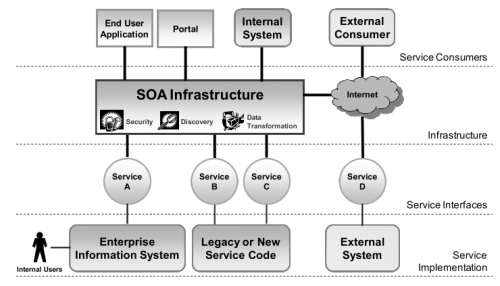
\includegraphics[width=0.8\linewidth]{images/SOA_GRAY.png}
\caption{SOA overview}
\label{fig:estilo-SOA}
\end{figure}


\subsection{Development life cycle}
\label{subsec:DevelopmentLifeCycle}
\todo{what is live-cycle development}

It is easy to find many software development life-cycle definition in the literature \cite{IEEE_Std_1074_1997,sommerville2007software,abrahamsson2003new,IEEE_Std_12207_2008,chatterjee2008software}, but defining a life cycle for agile software development is more difficult as agile in essence does not follow a rigorous process, as it can be seen in the Manifesto for agile software development \cite{alliance2001agile}. By the manifesto it is possible to see that processes, tools, comprehensive documentation, negotiation of contracts, and following a plan is not the most important, so it is possible to understand why it is difficult to find a well defined life cycle that synthesizes the agile way of developing software. 

On the other hand, there are some processes models to create \acrfull{SOA} applications as it is possible to see in \citet{Lane2011} such as Collaborative modeling (\todo{S22}), Semantic modeling (\todo{S37}), SOMA \cite{ArsanjaniSOMA2006}, Context aware (\todo{Context aware}), Web based (\todo{Web based}) and so on. In order to classify the processes into groups of related processes the authors used reciprocal translation \cite{noblit1988meta} and they synthesises the result in to a service development process meta-model, that present the following phases: analysis and design, construction and testing, deployment and provisioning and, execution and monitoring. This meta-model is similar to a map from a mapping study as outlined by \cite{budgen2008using,Petersen2008}.


\section{Research Method}
\label{sec:ResearchMethod}
In this this \acrfull{SLR} it was used the guidelines proposed by \citet{Kitchenham2004} and \citet{Kitchenham2007} and thus, the next steps where followed:

\begin{enumerate}
\item Planning the review:
	\begin{enumerate}[a)] % a), b), c), ...
	\item Identification of the need for a review
    \item Developing a review protocol
	\end{enumerate}
\item Conducting the review:
	\begin{enumerate}[a)] % a), b), c), ...
	\item Identification of research
    \item Selection of primary studies
    \item Study quality assessment
    \item Data extraction \& monitoring
    \item Data synthesis
	\end{enumerate}
\item Reporting the review
\end{enumerate}

A review protocol is a written plan that is completed before the review begins and it describes every aspect of the review from the background, the rationale for the survey, to the final report. A predefined protocol reduce the possibility researcher bias and provides a means by which the review itself can be repeated or updated at a later date to include subsequent publications  \cite{Lane2011,Kitchenham2004}. According to \citet{Kitchenham2004} the background is the rationale for the survey, explain the need for the review. In this paper the background is showed in the section \ref{sec:Background}. In the following subsections, it is presented the elements of the review according to the developed review protocol and some additional planning information.


\subsection{Research questions}
\label{subsec:ResearchQuestion}
As proposed by \cite{Kitchenham2007} the primary and secondaries research questions would elaborated for this study:
\begin{enumerate}
\item Primary Research Question (RQ01): What Agile processes are proposed for developing SOA Applications?
	\begin{itemize}
	\item Population: all roles in software development process;
    \item Intervention: agile Processes for development SOA applications.
    \item Control: Processes for traditional software development;
    \item Outcomes: set of Agile frameworks, models and techniques for developing SOA applications.
	\end{itemize}
\item Research Question (RQ02): What stages of the agile life cycle are the studies covering?
\item Research Question (RQ03): What common principles of \acrfull{SOA} are the studies covering?
\end{enumerate}

The RQ02 and RQ03 research questions complement the RQ01 research question. The research question RQ01 tries to answer what kind of contribution the studies bring, process, method, tool, etc., and the type of research approach, validation research, evaluation research, solution proposal, philosophical papers, opinion papers, or experience Papers \cite{wieringa2006requirements}. In addition, the RQ02 research question seeks to identify at which stage of the life cycle is the focus of the studies (see subsection \ref{subsec:AgileDevelopment}) and the RQ03 research question is concerned with identifying how common principles of \acrshort{SOA} are addressed in the studies (see subsection \ref{subsec:SOA}).

\todo{see \citet{Petersen2008} about a figure to RQ01}


\subsection{Search string and data sources}
\label{subsec:SearchStringDataSources}

To compose the search string the main words and synonyms were identified. Table \ref{tab:SearchSynonyms} describes these synonyms. At first, we tried to use other synonyms, such as \acrfull{XP}, SCRUM, Lean, and Crystal, but these synonyms did not add much, and sometimes brought undesirable works. In addition to the selected synonyms, the words "architecture", "computing", "system", and "application" were added to limit the result only to the type of study desired.

\begin{table}[ht]
\begin{tabular}{lll}
\hline
Agile Development & & Service-oriented Architecture \\ \hline
Agile Method & & SOA \\
Agile Programming & & SBA\footnote{\acrfull{SBA}} \\
Agile Process & & SOC\footnote{\acrfull{SOC}} \\
Agile Practice & & Webservice \\
Agile Requirement & & REST\footnote{\acrfull{REST}} \\
Agile Technique & & SOAP\footnote{\acrfull{SOAP}} \\
 & & Service-based \\ \hline
\end{tabular}
\caption{Search synonyms}
\label{tab:SearchSynonyms}
\end{table}

All of the used electronic data sources work with a well know structure to ask about electronic papers, using the operator `OR' to include synonyms for each search term, and the operator `AND' to link together each set of synonyms. Thus, the search string used was:
((
\textit{SOA} OR \textit{SBA} OR \textit{SOC} OR \textit{webservice*} OR \textit{``web service''} OR \textit{``web services''} OR \textit{REST} OR \textit{SOAP} 
OR 
((\textit{``software-oriented''} OR \textit{``Software oriented''}) AND (\textit{architecture} OR \textit{computing})) 
OR 
((\textit{``service-based''} OR \textit{``service based''}) AND (\textit{application*} OR \textit{system})
)) 
AND 
(\textit{``AGILE DEVELOPMENT''} OR \textit{``AGILE MANUFACTURING''} OR \textit{``AGILE METHOD''} OR \textit{``AGILE PROGRAMMING''} OR \textit{``AGILE PROCESS''} OR \textit{``AGILE PRACTICE''} OR \textit{``AGILE REQUIREMENT''} OR \textit{``AGILE TECHNIQUE''}))

As it is possible to see within the selection's criteria, table \ref{tab:StudySelectionCriteria}, it was chosen to work only with electronic data sources, so table \ref{tab:DataSources} lists those that were used. Each data source has its own peculiarity to do the search, so the search string above needed to be adapted for each case, but without losing its essence.

\begin{table}[ht]
\begin{tabular}{lll}
\hline
Source &  & URL \\ \hline
IEEE &  & \url{http://ieeexplore.ieee.org} \\
ACM &  & \url{http://portal.acm.org} \\
Web of Science &  & \url{http://www.isiknowledge.com} \\
Springer &  & \url{http://www.springerlink.com} \\
Science Direct &  & \url{http://www.sciencedirect.com} \\
Scopus &  & \url{https://www.scopus.com} \\ \hline
\end{tabular}
\caption{Data sources}
\label{tab:DataSources}
\end{table}

\subsection{Study selection, data extraction and quality assessment}
\label{subsec:StudySelAndExt}

All electronic data sources used in this work provide advanced tools that allow the definition of other parameters at the time of the search. Even though the original data source tool does not provide all the necessary features, some parameters are easy to identify in standalone tools, such as an electronic data sheet. Some selection criteria used in this work fit this type of parameters, which can be seen in the section "Criteria for inclusion of studies / Automatically identified" in the table \ref{tab:StudySelectionCriteria}.

The other criteria for inclusion and exclusion of studies were identified through a careful reading of the authors title, abstract and keywords. Some studies were excluded late, during the data extraction phase, when the studies were read integrally. This was because a conservative criterion was used in this selection phase: \textit{`in case of doubt the study remains'}.

During the extraction phase the selected studies were assessed in order to identify the degree to adjustment of the purposes of the \acrshort{SLR}.


\begin{table}[ht]
%\resizebox{\textwidth}{!}{%
%\begin{adjustbox}{max width=\textwidth}
%\begin{tabular}{l}
\begin{tabularx}{.9\textwidth}{Xl}
\hline
Studies' inclusion criteria  \\ \hline
- Automatically identified \\
\hspace{1cm}  - Published and available in electronic data sources \\
\hspace{1cm}  - Only articles and reviews \\
\hspace{1cm}  - Contain search keywords in the title, abstract or author keywords \\
\hspace{1cm}  - In English \\
\hspace{1cm}  - All publication years \\
- Personally identified \\
\hspace{1cm}  - About SOA development using Agile Development Method \\
\hspace{1cm}  - Have to be more than four pages \\
\hline
Studies' exclusion criteria \\ \hline
- Studies that cite SOA and Agile although it isn't the main purposes to explain about development SBA using agile \\
- Papers which are obviously not related to the research questions in this protocol \\
- Duplicate publications on the same approach  \\ \hline
\end{tabularx}
%\end{tabular}
%}
%\end{adjustbox}
\caption{Study selection criteria}
\label{tab:StudySelectionCriteria}
\end{table}

\begin{table}[ht]
\begin{tabularx}{.9\textwidth}{lXlXlX}
\hline
Data field & Porpose & \begin{tabular}[c]{@{}l@{}}Research \\ questions\end{tabular} \\ \hline
Reviewer & Name of reviwer & RQ1 \\
Title & Name of study & RQ1 \\
Authors & Study authors & RQ \\
Publication source & Where the paper was published, name of journal, conference, etc. & RQ \\
Publication type & Is the paper a conference paper, journal paper, etc.? & RQ \\
Year of publication & When study was published & RQ \\
Primary/secondary & Does the study use primary or secondary data? & RQ \\
Study type & Type of research methods used & RQ \\
Study population & Study participants, students, academics, industry experts, etc. & RQ \\
Research question & Research question(s) of the study & RQ \\
Study focus & Primary objective of the study & RQ \\
Processes & Process described in the study & RQ \\
Findings/conclusions & Main conclusions from the study & RQ \\
IS valid & Was it a valid study? & RQ \\ \hline
\end{tabularx}%
\caption{Data extraction fields}
\label{tab:DataExtractionFields}
\end{table}

\subsection{Data synthesis strategy}
\label{subsec:DataSynthesis}
\todo{todo}


\section{Research Review}
\label{sec:Review}
Begening apllying the research method, it ware found xxx primary studies, that was reduced to yyy after the phase of selection and extraction.

\todo[inline]{Table of final articles}





\todo[inline]{Summary of selected studies}

\todo[inline]{Question address}



\section{Discussion}
\label{sec:Discussion}
Discussion xxx

To accomplish this work, it was necessary to define a development life-cycle to evaluate the selected works. Thus, it was used the concepts of \cite{papazoglou2006service} which attempt to compare a complete life cycle and its use in the most prominent development methods that claim to be agile. In this context, the development life-cycle phases are project inception, requirements specification, design, coding, unit test, integration test, system test, acceptance test, and maintenance. For the purposes of this paper, only the middle bar in Figure \todo{put figure} is important. The middle bar refers to the software development life-cycle analysis, where the gray bar indicates that the phase is supported by the agile method and the white bar indicates that the phase is not supported.


%%%\IEEEtriggeratref{16}

\bibliographystyle{bibtex/bib/IEEEtran}
\bibliography{bibtex/bib/IEEEabrv.bib,bibtex/bib/Mendeley.bib}{}

\end{document}
